%%% Local Variables:
%%% mode: latex
%%% TeX-master: "../main_file"
%%% End:

\section{Algorithmes de filtrage basés sur le Time-Table}

La section suivante présente plusieurs algorithmes de filtrage pour le
\CECSP. Tous ces algorithmes utilisant une adaptation du Time-Table
pour le \CUSP, nous commençons donc par présenter brièvement comment
ce raisonnement est modifié pour être adapté dans le cadre du \CECSP.
Puis, nous présentons deux autres algorithmes permettant
de réduire l'ensemble des valeurs possibles pouvant être prises par
chaque variable. Le premier est adapté du Time-Table disjonctif pour
le \CUSP~\cite{Gay2015} et le dernier utilise une combinaison entre
problème de flots et profil obligatoire.

\subsection{Le Time-Table}
\index{Time-Table!CECSP}
Comme pour le \CUSP, le Time-Table pour le \CECSP~se base sur la
notion de partie obligatoire des activités, i.e. l'intervalle pendant
lequel une activité est en cours d'exécution dans tous les
ordonnancements réalisables. Cependant, comme dans le
cas du \CECSP, nous ne connaissons pas la durée exacte d'une activité,
nous utilisons une borne inférieure sur sa durée pour calculer la date
de début au plus tard, $\LS$, et la date de fin au plus tôt,
$\EE$. Pour calculer cette borne, remarquons que la configuration
permettant de finir une activité le plus rapidement possible, est
celle où l'activité est exécutée à son rendement $\bmax$. De ce fait,
une borne inférieure sur la durée de l'activité vaut
$W_i/f_i(\bmax)$. Nous pouvons donc calculer la date de début au plus
tard de l'activité, $\LS=d_i-W_i/f_i(\bmax)$, et sa date de fin au
plus tôt, $\EE=r_i+W_i/f_i(\bmax)$. La partie obligatoire d'une
activité $i$ est alors définie de a même manière que pour le \CUSP,
i.e la partie obligatoire de $i$ est l'intervalle $[\LS,\EE]$ (cf. figure~\ref{fig_mand_CECSP}). 

Cependant, dans le cas où $\LS \le \EE$, i.e. où l'activité possède
une partie obligatoire, nous pouvons seulement déduire que l'activité
$i$ va consommer au moins une quantité $\bmin$ de la ressource durant
toute sa partie obligatoire, et ce, quelque soit le moment où
l'activité est ordonnancée. La notion de profil obligatoire de la
ressource est donc légèrement différente de celle définie pour le
\CUSP~(cf. définition~\ref{def:profil_oblig},
page~\pageref{def:profil_oblig}). 

\begin{defi}
Le profil obligatoire d'une ressource $TT_{\A}$ dans le cas du
\CECSP~est définie de la façon suivante: 
\[TT_{\A}(t)=\sum_{\substack{i \in \A\\\LS \le t \le \EE}} \bmin\quad
  \forall t \in \H\]
Le problème est donc insatisfiable dans le cas où $\exists t \in \H\
:\ TT_{\A}(t) > R$
\end{defi}

\begin{ex}
Considérons l'activité suivante: 

\vspace{-0.5cm}
\begin{center}
  \begin{tabular}{|P{1cm}P{1cm}P{1cm}P{1cm}P{1cm}P{1cm}|}
    \hline
    \ES & \LE & W_i & \bmin & \bmax & f_i(b)\\
    \hline
    1 & 14 & 72 & 2 & 5 & b+3\\
    \hline
  \end{tabular}
\end{center}

Nous pouvons calculer sa date de début au plus tard,
$\LS=d_i-W_i/f_i(\bmax)=14 - 72/8 =5$, ainsi que sa date de fin au
plus tôt, $\EE=r_i+ W_i/f_i(\bmax)=1 + 72/8 =10$. Comme $\EE > \LS$,
l'activité possède une partie obligatoire qui est l'intervalle
$[5,10]$ (voir
figure~\ref{fig_mand_CECSP_a},~\ref{fig_mand_CECSP_b}). Cependant,
nous pouvons seulement en déduire que l'activité sera en cours dans
cet intervalle et ,grâce à la borne inférieure sur la quantité de
ressource que peut consommer l'activité durant son exécution, nous
pouvons déduire que, sur l'intervalle $[\LS,\EE]$, l'activité est au
moins exécutée à $\bmin$ (voir figure~\ref{fig_mand_CECSP_c}).
  
\begin{figure}[htb!]
\vspace{-0.8cm}
\subcaptionbox{Ordonnancement au plus tôt\label{fig_mand_CECSP_a}}[0.3\linewidth]{
    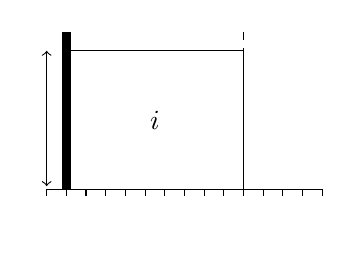
\begin{tikzpicture}
      [xscale=0.25, yscale= 0.4,node distance=0.5cm]
      \node (sil) at (1,0) {} ;
      \node (eil) at (10,0) {} ;
      \node [below of=eil,node distance=0.63cm]  {$\EE$};
      \draw (sil.center) node[below=0.2cm] {$\ES$};
      
      \draw (0,0) -- (14,0);
      \draw[line width=3pt] (1,0) -- (1,5);
      
      \draw[<->] (0,0.1) -- (0,4.4) node[midway,left] {$\bmax$};
      \draw (1,0) rectangle (10,4.4) node[midway] {$i$};

      \draw[dashed] (10,0) -- (10,5);

      \foreach \i in {0,...,14} {
        \draw (\i,0)  -- (\i,-0.2);
      }
    \end{tikzpicture}
}
\hfill
\subcaptionbox{Ordonnancement au plus tard\label{fig_mand_CECSP_b}}[0.3\linewidth]{
    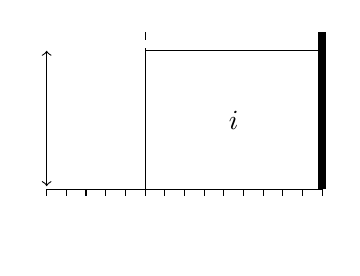
\begin{tikzpicture}
      [xscale=0.25, yscale= 0.4,node distance=0.5cm]
      \node (sir) at (5,0) {} ;
      \node (eir) at (14,0) {} ;
      \node[below of= sir,node distance=0.63cm] {$\LS$};
      \draw (eir.center) node[below=0.2cm] {$\LE$};
      
      \draw (0,0) -- (14,0);
      \draw[line width=3pt] (14,0) -- (14,5);
      
      \draw[<->] (0,0.1) -- (0,4.4) node[midway,left] {$\bmax$};
      \draw (5,0) rectangle (14,4.4) node[midway] {$i$};

      \draw[dashed] (5,0) -- (5,5);

      \foreach \i in {0,...,14} {
        \draw (\i,0)  -- (\i,-0.2);
      }
    \end{tikzpicture}
}
\hfill
\subcaptionbox{Ordonnancement réalisable à $\bmin$ dans
  $[\LS,\EE]$ \label{fig_mand_CECSP_c}}[0.3\linewidth]{ 
    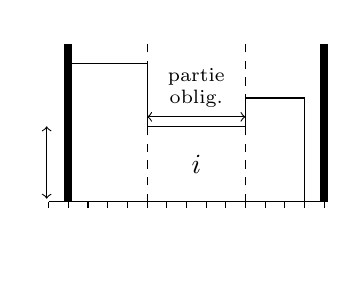
\begin{tikzpicture}
      [xscale=0.25, yscale= 0.4,node distance=0.5cm]
      \node (sir) at (5,0) {} ;
      \node (eil) at (10,0) {} ;
      \node [below of=eil,node distance=0.63cm]  {$\EE$};
      \node[below of= sir,node distance=0.63cm] {$\LS$};
      \draw[<->] (5,2.7) -- (10,2.7) node[midway,above,text width=1.4cm]
      {\begin{center} \scriptsize partie oblig. \end{center}};
      
      \draw[white] (5,0) rectangle (10,2.4) node[midway,color=black] {$i$};
           
      \draw (1,4.4) -- (5,4.4) -- (5,2.4) -- (10,2.4) -- (10,3.3) --
      (13,3.3) -- (13,0);
      
      \draw (0,0) -- (14,0);
      \draw[line width=3pt] (1,0) -- (1,5);
      \draw[line width=3pt] (14,0) -- (14,5);
      
      \draw[<->] (-0.1,0.1) -- (-0.1,2.4) node[midway,left] {$\bmin$};
    


      \draw[dashed] (5,0) -- (5,5);
      \draw[dashed] (10,0) -- (10,5);

      \foreach \i in {0,...,14} {
        \draw (\i,0)  -- (\i,-0.2);
      }
    \end{tikzpicture}
}
\caption{Partie obligatoire d'une activité $i$}
\label{fig_mand_CECSP}
\end{figure}
\end{ex}

Le profil obligatoire peut aussi être calculé en $O(n)$ à l'aide d'un
algorithme de balayage en triant au préalable les activités par date
de début au plus tard et date de fin au plus tôt (voir
algorithme~\ref{algo_profil}).

Nous détaillons maintenant l'adaptation du Time-Table disjonctif au
\CECSP. 

\subsection{Le Time-Table disjonctif}

Le second algorithme de filtrage proposé repose sur un raisonnement
appelé Time-Table disjonctif et utilisé, en premier lieu, pour le
\CUSP (cf. paragraphe~\ref{sec:mix_CUSP}). Ce dernier repose sur le
raisonnement Time-Table décrit précédemment et sur le raisonnement
disjonctif.

Le raisonnement disjonctif dans le cadre du \CECSP, est très similaire
à celui défini pour le \CUSP. La différence repose sur la construction
d'ensembles disjonctifs. Dans le cas du \CECSP, un couple d'activité
($i,j)$ sera dit disjonctif si $\bmin+\bmin[j] >R$. Dans ce cas, nous
savons que: 
\begin{itemize}
\item l'activité $i$ doit commencer après l'activité $j$, ou, 
\item l'activité $i$ doit finir avant l'activité $j$.  
\end{itemize}

Cette propriété permet d'améliorer les bornes des variables de
début et fin d'une activité. La règle de filtrage est ensuite la même
que dans le cas du \CUSP. 

Cette contrainte nous permet, entre autre, d'ajuster la date de début
au plus tôt de $j$. En effet, $\ES[j] \le
\EE$ et $\LS \le \EE[j]$ implique que $j$ doit commencer après la fin
de l'activité $i$ (voir figure~\ref{fig_disj}). De ce fait, la début
de $j$ ne peut arriver avant la date de fin au plus tôt de $i$, et
donc: $\ES[j] \ge \EE$.

\begin{figure}[!htb]
  \centering 
  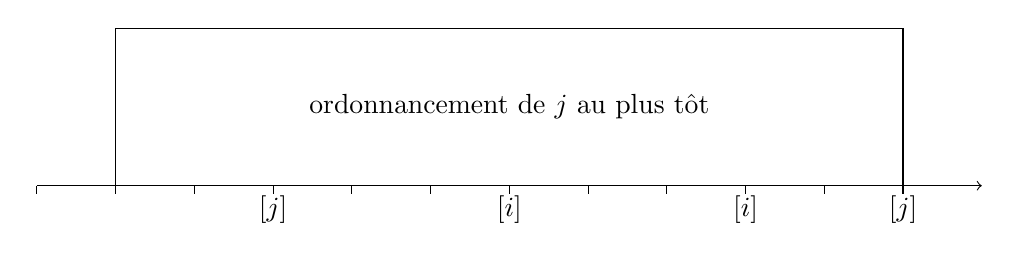
\begin{tikzpicture}
    \node (O) at (0,0) {};
    \draw[->] (0,0) -- (12,0);
    \foreach \i in {0,...,11}
    {\draw (\i,0) -- (\i, -0.1) ;}

    \draw (1,0) node[below] {$\ES$};
    \draw (3,0) node[below] {$\ES[j]$};
    \draw (6,0) node[below] {$\EE[i]$};
    \draw (9,0) node[below] {$\LS[i]$};
    \draw (11,0) node[below] {$\EE[j]$};

    
    \draw (1,0) rectangle (11,2) node[midway] {ordonnancement de $j$
      au plus tôt};
 \end{tikzpicture}
  \caption{Raisonnement disjonctif}
  \label{fig_disj}
\end{figure}



\subsection{Le Time-Table basé sur les flots}


